\documentclass[english,course]{Notes}

\title{Lecture 21: Unsupervised Learning}
\subject{Theory of Machine Learning}
\author{Instructor: Aditya Bhaskara \qquad Scribe: Jake Pitkin}
\date{29}{03}{2017}
\place{{\bf CS 5966/6966: Theory of Machine Learning}}

\usepackage{float}
\newcommand{\Tr}{\text{Tr}}
\newcommand{\iprod}[1]{\langle #1 \rangle}
\newcommand{\R}{\mathbb{R}}
\renewcommand{\norm}[1]{\lVert #1 \rVert}
\newcommand{\su}[1]{^{(#1)}}
\newcommand{\bu}{\mathbf{u}}
\renewcommand{\deg}{\text{deg}}

\begin{document}
\vspace{-10pt}
\begin{abstract}
In this lecture, we introduce the concept of unsupervised learning by looking at a commonly used and broad statistical technique called clustering. We look at using a mixture of Gaussian distributions to cluster data points as well as the \textit{k}-means optimization problem and algorithm.
\end{abstract}

%%% Notes start in detail
\section{Introduction}

Similar to other forms of learning we have studied, the goal of unsupervised learning is to discover patterns in a set of data. It is unique from supervised learning or reinforcement learning in two main ways. First, data points do not come with labels and the goal is rarely to just classify the data. Second, there is no "ground truth" or evaluation of accuracy as the data points are unlabeled. Unsupervised learning is desirable as annotated data is rare and expensive to produce. In contrast, unlabeled data is typically plentiful and much easier to obtain in large quantities.

\section{Motivating Examples}

As motivation for unsupervised learning techniques, we will briefly look at three example applications.

\textbf{Movie Recommendations}

Consider a service such as Netflix that is interested in making movie recommendations. They could keep a matrix of \textit{movies} $\times$ \textit{users} where the entries in the matrix are say a rating on a scale of $1-5$. As there exists a large number of \textit{movies} and \textit{users} this will be a sparse matrix.

$$\begin{bmatrix}
  & user_1  & \dots & \dots & user_n\\
    movie_1 & & 3\\
    \vdots  \\
    \vdots  & & & & 4\\
    movie_m & 2
\end{bmatrix} $$ 

Now say we want to determine the likelihood that $user_i$ would enjoy $movie_j$. By using the data points we do have, we could look at the attributes of those movies and users in an attempt to find a hidden structure in the data. This hidden structure could then be used to guide our recommendation process. \\

\textbf{Cocktail Party Problem}

Imagine being at a cocktail party where the room is noisy from multiple separate conversations occurring simultaneously. There is a spy in the room with a microphone that is picking up the superposition of a whole bunch of signals. After collecting this audio data, the goal of the spy is to break up the signals into "components" in an attempt to isolate each of the individual conversations. \\

\textbf{Sparse Coding}

In the field of neuroscience, there is work being done to understand how our brains encode sensory input of images. Each image is encoded as a sparse combination of a few basic patterns. Given visual signals, the brain finds a small set of these patterns such that the images we see can be formed as a sparse combination of these basic patterns. This allows the images to be understood by the brain using a relatively small number of neurons.

\section{Unsupervised Learning}

In unsupervised learning, we assume the data points are generated by some random process with a "few parameters" that are unknown. This assumption is called a generative assumption as we are assuming the data is produced by a unknown generative model. We have seen generative models before in supervised learning and they are not unique to unsupervised learning. \\

The goal of unsupervised learning is to identify these hidden parameters. These parameters could be central points or centroids and how these points relate to nearby points. If we identify these parameters, we could cluster the data into groups. We are operating under the assumption that the data has some underlying explanation. Additionally, there is no "ideal" model and we can overfit the data or underfit the data depending on the model complexity. 

\section{Clustering}

Clustering is a widely used and broad technique to understand unlabeled data. Consider a set of points $\mathcal{X} \in \mathbb{R}$
\begin{figure}[H]
  \centerline{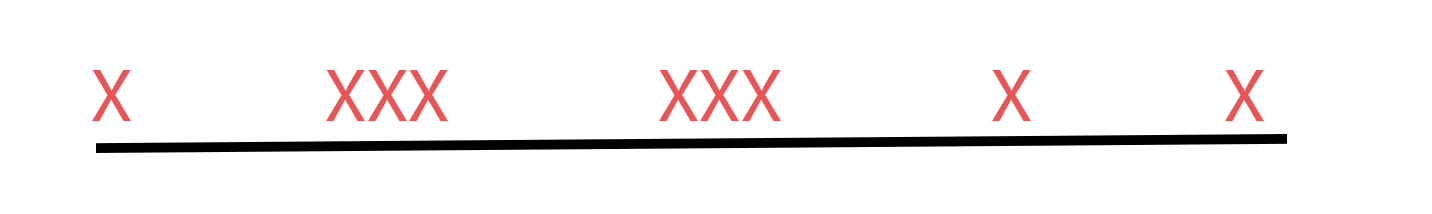
\includegraphics[width=0.7\linewidth]{fig1.png}}
\end{figure}

As you could imagine, you could use a say degree five polynomial to closely fit the data points. The downside being this complicated model is overfitting the given data and it is likely to generalize poorly on future data points. What if instead we used a mixture of Gaussian distributions as a way to model the data \\ 

 Let's first consider using the Gaussian distribution to define the probability density of a data point $x$ as a way to cluster data into groups. The Gaussian distribution is defined by the mean $\mu$ and the variance $\sigma^2$ as such

\begin{equation}
\label{eq:transition1}
f(x \ \vert \ \mu , \sigma^2) = \frac{1}{\sqrt{2 \pi \sigma^2}} e^{-\frac{(x - \mu)^2}{2 \sigma^2}}
\end{equation}



\section{The \textit{k}-Means Algorithm}

\section{Conclusion}
\end{document}
